\documentclass[../notes.tex]{subfiles}

\pagestyle{main}
\renewcommand{\chaptermark}[1]{\markboth{\chaptername\ \thechapter\ (#1)}{}}

\begin{document}




\chapter{From Classical to Quantum Mechanics}
\section{Blackbody Radiation}
\begin{itemize}
    \item \marginnote{9/27:}The surface of a hot body emits energy in the form of EM radiation.
    \item Changes that occur with temperature:
    \begin{itemize}
        \item If less than $\SI{500}{\celsius}$, we have IR Radiation (heat).
        \item If $\SIrange{500}{600}{\celsius}$, we have visible radiation (a glowing body).
        \item If $\SI{5000}{\celsius}$, we have a "white hot" body (short wavelength).
    \end{itemize}
    \item As a body gets hotter, it emits shorter wavelength radiation.
    \item \textbf{Stefan-Boltzmann law}: The the total emissive power $R$ (recall that power is en / time) of a blackbody (BB) is given by
    \begin{equation*}
        R(T) = \sigma T^4
    \end{equation*}
    where $\sigma\approx\SI{5.67e-8}{\watt\per\square\meter\per\kelvin\tothe{4}}$ is \textbf{Stefan's constant}.
    \begin{itemize}
        \item Work done by Stefan and Boltzmann (c. 1870 / 1884, respectively).
    \end{itemize}
    \item \textbf{Wien's 1st Law}: The wavelength for maximum emissive power obeys the equation
    \begin{equation*}
        \lambda_\text{max}T = b
    \end{equation*}
    where $b=\SI{2.898e-3}{\meter\kelvin}$ is \textbf{Wein's displacement constant}. \emph{Also known as} \textbf{Wien's displacement law}.
    \begin{figure}[h!]
        \centering
        \begin{tikzpicture}
            \footnotesize
            \draw [<->] (0,4.5) -- node[left]{$R(\lambda,T)$} (0,0) -- node[below=2mm]{$\lambda\ (\si{\micro\meter})$} (7.5,0);
            \foreach \x in {1,...,7} {
                \draw (\x,0.1) -- ++(0,-0.2);
            }
            \foreach \y in {1,...,4} {
                \draw (0.1,\y) -- ++(-0.2,0);
            }
            
            \begin{scope}[xscale=1.8]
                \draw [blx,thick,samples=100,smooth,/pgf/fpu,/pgf/fpu/output format=fixed] plot[domain=0.1:4] (\x,{5*10^2/(\x^5*(e^(9900/(2000*\x))-1))});
                \draw [grx,thick,samples=100,smooth,/pgf/fpu,/pgf/fpu/output format=fixed] plot[domain=0.1:4] (\x,{5*10^2/(\x^5*(e^(9900/(1750*\x))-1))});
                \draw [orx,thick,samples=100,smooth,/pgf/fpu,/pgf/fpu/output format=fixed] plot[domain=0.1:4] (\x,{5*10^2/(\x^5*(e^(9900/(1500*\x))-1))});
                \draw [rex,thick,samples=100,smooth,/pgf/fpu,/pgf/fpu/output format=fixed] plot[domain=0.1:4] (\x,{5*10^2/(\x^5*(e^(9900/(1000*\x))-1))});
        
                \draw [semithick] (0.997,3.667) node[above right]{$\lambda_\text{max}$} -- ++(0,-0.2);
                \draw [semithick] (1.139,1.93) -- ++(0,-0.2);
                \draw [semithick] (1.329,0.946) -- ++(0,-0.2);
                \draw [semithick] (1.994,0.211) -- ++(0,-0.2);
            \end{scope}
    
            \begin{scope}[xshift=6cm,yshift=3cm]
                \node at (0,1.2) {${\color{blx}\blacksquare}=\SI{2000}{\kelvin}$};
                \node at (0,0.8) {${\color{grx}\blacksquare}=\SI{1750}{\kelvin}$};
                \node at (0,0.4) {${\color{orx}\blacksquare}=\SI{1500}{\kelvin}$};
                \node at (0,0) {${\color{rex}\blacksquare}=\SI{1000}{\kelvin}$};
            \end{scope}
        \end{tikzpicture}
        \caption{Wein's 1st Law.}
        \label{fig:WeinLaw1}
    \end{figure}
    \item Area under the curve (found with integration) is the total emissive power.
    \item We now change variables from emissive power $R$ to energy density $\rho$ in the BB cavity.
    \begin{equation*}
        \rho(\lambda,T) = \frac{4}{c}R(\lambda,T)
    \end{equation*}
    \item Wien's 2nd Law (1893): The energy density must have a functional relationship with the following form.
    \begin{equation*}
        \rho(\lambda,T) = \frac{f(\lambda T)}{\lambda^5}
    \end{equation*}
    \begin{itemize}
        \item $f(\lambda T)$ cannot be determined from thermodynamics. Thus, something else is needed!
    \end{itemize}
    \item Lord Rayleigh and his graduate student Jeans (1899) propose a solution.
    \begin{itemize}
        \item EM: The thermal radiation within a cavity must exist in the form of standing waves.
        \item RJ showed that the number $n$ of standing waves per unit volume, per wavelength has the following form.
        \begin{equation*}
            n(\lambda) = \frac{8\pi}{\lambda^4}
        \end{equation*}
        \item If $\bar{\epsilon}$ is the average energy in the mode with wavelength $\lambda$, then
        \begin{equation*}
            \rho(\lambda,T) = \frac{8\pi}{\lambda^4}\bar{\epsilon}
        \end{equation*}
        \item Waves come from atoms in the walls of the BB cavity, which act as linear harmonic oscillators at a frequency $\nu=c/\lambda$.
        \item Assuming thermal equilibrium, we obtain
        \begin{align*}
            \bar{\epsilon} &= \frac{\int_0^\infty\epsilon\e[-\epsilon/kT]}{\int_0^\infty\e[-\epsilon/kT]}\\
            &= -\pdv{\beta}\ln\left( \int_0^\infty\e[-\beta\epsilon]\dd{\epsilon} \right)\\
            &= \frac{1}{\beta}\\
            &= kT
        \end{align*}
        where $k$ is the Boltzmann constant.
        \begin{itemize}
            \item Basically, we sum all energies $\epsilon$, weighted by the probability $\e[-\epsilon/kT]$ of the energy existing, and divided by the total energy.
            \item The first equation is equivalent to the second with $\beta=1/kT$.
        \end{itemize}
        \item Therefore,
        \begin{equation*}
            \rho(\lambda,T) = \frac{8\pi kT}{\lambda^4}
        \end{equation*}
    \end{itemize}
    \item UV catastrophe: Rayleigh's formula diverges from the experimental data for short wavelength.
    \begin{itemize}
        \item The above formula diverges to $+\infty$, driven by the $\lambda^4$ term in the denominator, as $\lambda\to 0$. However, the amount of radiation of shorter wavelengths should decrease past a point, as seen in Figure \ref{fig:WeinLaw1}.
    \end{itemize}
    \item Max Planck comes in, proposes an idea to the German acacdemy that's so radical, they think he's insane, but he's actually right and it lays a key idea for quantum mechanics.
    \item Planck's key insight: The energy levels of the oscillators are not continuous, but are quantized.
    \begin{itemize}
        \item So we can't actually take an integral as Rayleigh did; we have to take an infinite series.
        \item In reality,
        \begin{align*}
            \bar{\epsilon} &= \frac{\sum_{n=0}^\infty n\epsilon_0\e[-\beta n\epsilon_0]}{\sum_{n=0}^\infty\e[-\beta n\epsilon_0]}\\
            &= \frac{\epsilon_0}{\e[\beta\epsilon_0]-1}
        \end{align*}
        \item Thus,
        \begin{equation*}
            \rho(\lambda,T) = \frac{8\pi\epsilon_0}{\lambda^4(\e[\epsilon/kT]-1)}
        \end{equation*}
        \item But to satisfy Wien's 2nd law, we must let $\epsilon_0\propto 1/\lambda$. More specifically, $\epsilon_0=hc/\lambda=h\nu$, where $h$ is Planck's constant.
        \begin{itemize}
            \item This setup allowed us to get an accurate value for Planck's constant for the first time in history.
        \end{itemize}
        \item Planck's theory predicts the data of Figure 1.
    \end{itemize}
    \item A perfect blackbody absorbs and emits radiation at all frequencies.
    \begin{itemize}
        \item A star is pretty close to a blackbody. The graphite in a pencil is 97\% a blackbody. We are all blackbodies.
        \item The entire universe can be viewed as a blackbody.
    \end{itemize}
    \item Princeton and Bell Labs telescopes find \textbf{Cosmic Background Radiation} (A. A. Penzias and R. W. Wilson, 1964).
    \begin{itemize}
        \item Background radiation from the universe itself.
        \item $\lambda_\text{max}=\SI{7.35}{\centi\meter}$.
        \item Isotropic radio signal, that comes form everywhere.
        \item From this, you can workout the temperature of the universe from Wein's first law.
        \item Thus, the whole universe is a blackbody with a temperature of approximately $\SI{3}{\kelvin}$.
    \end{itemize}
\end{itemize}



\section{Photoelectric Effect and Bohr Atom}
\begin{itemize}
    \item \marginnote{9/29:}In 1887, Hertz shines UV light at electrodes and observes a spark.
    \begin{itemize}
        \item In 1900, Lenard shows that electrons are ejected from the metal surface of the electrodes.
    \end{itemize}
    \item Experimental setup:
    \begin{figure}[h!]
        \centering
        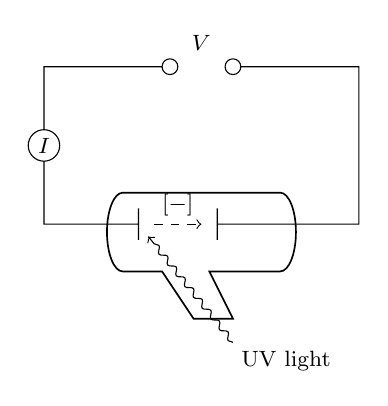
\begin{tikzpicture}
            \footnotesize
            \draw
                (0.4,2) circle (1mm)
                (-0.4,2) circle (1mm)
                (-2,1) circle (2mm) node{$I$}
                (-0.5,2) -- (-2,2) -- (-2,1.2) (-2,0.8) -- (-2,0) -- (-0.8,0) (0.2,0) -- (2,0) -- (2,2) -- (0.5,2)
                (-0.8,-0.2) -- ++(0,0.4) (0.2,-0.2) -- ++(0,0.4)
            ;
            \node at (0,2.3) {$V$};
    
            \draw [semithick] (1,0.4) -- ++(-2,0) arc[start angle=90,end angle=270,x radius=2mm,y radius=5mm] -- ++(0.5,0) -- ++(0.4,-0.6) -- ++(0.5,0) -- ++(-0.3,0.6) -- ++(0.9,0) arc[start angle=-90,end angle=90,x radius=2mm,y radius=5mm];
    
            \draw [decoration={snake,post length=3mm,amplitude=1pt,segment length=5pt},decorate,->,shorten >=2mm] (0.4,-1.5) node[below right]{UV light} -- (-0.8,0);
            \draw [dashed,->] (-0.6,0) -- node[above]{$\e[-]$} (0,0);
        \end{tikzpicture}
        \caption{Photoelectric effect experiment.}
        \label{fig:PEeffectExp}
    \end{figure}
    \begin{itemize}
        \item Shine UV light through a quartz crystal window so that it impinges on the left plate.
        \item This causes an electron to be ejected from the illuminated plate and cross the potential difference (recall that they didn't know about electrons at the time; they just knew something was happening).
        \item Increase the external potential until the spark goes away (gives some data about the energy of the electron).
    \end{itemize}
    \item Odd features:
    \begin{enumerate}
        \item There is a threshold frequency of radiation required to eject the electrons.
        \begin{itemize}
            \item You can shine as much light as you want below a certain frequency and nothing will happen.
            \item However, as soon as you reach that frequency, you get a spark.
        \end{itemize}
        \item The maximum kinetic energy (KE necessary to overcome the voltage PE???) depends linearly upon the frequency and is independent of the intensity.
    \end{enumerate}
    \item Einstein (1906) proposes that light consists of quanta called photons.
    \item If you assume this, Max KE obeys the following form.
    \begin{equation*}
        \frac{1}{2}mv_\text{max}^2 = h\nu-W
    \end{equation*}
    where the work function $W$ is the energy required to remove the photon from the metal.
    \begin{itemize}
        \item When $KE\to 0$, we obtain the threshold frequency
        \begin{equation*}
            \nu_\text{th} = \frac{W}{h}
        \end{equation*}
        required to remove an electron from the metal.
    \end{itemize}
    \item Millikan (1914-1917), hot off the success of the oil drop experiment, experimentally corroborates Einstein's theory at UChicago in Ryerson.
    \begin{itemize}
        \item Noting that $KE=eV$ as well where $e$ is the charge of an electron and $V$ is the stopping voltage, Millikan obtains
        \begin{equation*}
            V = \frac{h}{e}\nu-\frac{W}{e}
        \end{equation*}
        \item The slope of this linear data plot is $h/e$, and Millikan definitely knows the charge of the electron (!), so he can also measure Planck's constant this way.
        \item When Millikan gets the same value Planck got a different way, he corroborates Einstein's theory.
    \end{itemize}
    \item Thus, this quantization is not just one result, but is fundamental to our understanding of radiation.
    \item Bohr (1913) makes assumptions.
    \begin{enumerate}
        \item Circle orbits of electrons about the nucleus.
        \item Only certain stationary orbits are allowed.
        \item The electron radiates energy only during a transition between orbits.
        \item The orbital angular momentum is quantized: $L=\frac{nh}{2\pi}$ where $n\in\N$ is a quantum number.
    \end{enumerate}
    \item Assumption 1 is wrong.
    \item Two equations:
    \begin{itemize}
        \item Equation one: Coulomb attraction of the electron and proton (nucleus) is balanced by a centripetal acceleration.
        \begin{equation*}
            \frac{Ze^2}{4\pi\epsilon_0r^2} = \frac{mv^2}{r}
        \end{equation*}
        where $Z$ is the charge of the nucleus, and $e$ is the charge of an electron.
        \begin{itemize}
            \item This follows exactly from classical mechanics.
        \end{itemize}
        \item Equation two: Quantization of the orbital angular momentum:
        \begin{equation*}
            mvr = \frac{nh}{2\pi} = n\hbar
        \end{equation*}
        where $\hbar=h/2\pi$.
        \begin{itemize}
            \item This is a new development from quantum mechanics.
        \end{itemize}
    \end{itemize}
    \item We now solve the two equations for our two unknowns (the velocity and radius).
    \begin{align*}
        v &= \frac{Ze^2}{4\pi\epsilon_0\hbar n}&
        r &= \frac{4\pi\epsilon_0\hbar^2n^2}{Zme^2}
    \end{align*}
    \item It follows that the translational kinetic energy $T$ is given by
    \begin{align*}
        T &= \frac{1}{2}mv^2\\
        &= \frac{m}{2\hbar}\left( \frac{Ze^2}{4\pi\epsilon_0} \right)^2\frac{1}{n^2}
    \end{align*}
    \begin{itemize}
        \item This is the origin of the $1/n^2$ in the Bohr model.
    \end{itemize}
    \item With respect to potential energy, we also have
    \begin{align*}
        V &= -\frac{Ze^2}{4\pi\epsilon_0r}\\
        &= -\frac{m}{\hbar^2}\left( \frac{Ze^2}{4\pi\epsilon_0} \right)^2\frac{1}{n^2}
    \end{align*}
    \item It follows that the total energy $E$ is given by
    \begin{align*}
        E_n &= T+V\\
        &= -\frac{m}{\hbar^2}\left( \frac{Ze^2}{4\pi\epsilon_0} \right)^2\frac{1}{n^2}
    \end{align*}
    \item Thus, the reason we have discrete transitions is because the atom has discrete energy levels.
    \item Indeed, energy transitions are described by the following.
    \begin{equation*}
        E_b-E_a = hcR_0\left( \frac{1}{n_b^2}-\frac{1}{n_a^2} \right)
    \end{equation*}
    where $R_0$, the Rhydberg constant (observed by Rhydberg and his spectral lines far before Bohr, but applicable here), is all of the other constants swept together.
    \begin{itemize}
        \item Note that
        \begin{equation*}
            R_0 = \frac{m\left( \frac{e^2}{4\pi\epsilon_0} \right)^2}{4\pi c\hbar^3}
        \end{equation*}
        \item Thus, quantum mechanics exactly describes the spectral transitions experimentally described earlier.
    \end{itemize}
    \item Limitations of the Bohr model:
    \begin{enumerate}
        \item Assumption 1.
        \item Cannot be generalized to many electron atoms and models.
        \item No reliable way to predict the time dependence of events like the electron transitions.
    \end{enumerate}
    \item So the Bohr model brings us to the brink of being able to predict chemistry, but we still need to go a bit further.
\end{itemize}



\section{Chapter 1: The Dawn of the Quantum Theory}
\emph{From \textcite{bib:McQuarrieSimon}.}
\begin{itemize}
    \item \marginnote{9/28:}\textbf{Blackbody}: A body which absorbs and emits all frequencies. \emph{Also known as} \textbf{ideal body}.
    \item "Many theoretical physicists tried to derive expressions consistent with these experimental curves of intensity versus frequency [see Figure \ref{fig:WeinLaw1}], but they were all unsuccessful. In fact, the expression that is derived according to the laws of nineteenth century physics is" as follows \parencite[3]{bib:McQuarrieSimon}.
    \item \textbf{Rayleigh-Jeans law}: The equation
    \begin{equation*}
        \dd{\rho(\nu,T)} = \rho_\nu(T)\dd{\nu} = \frac{8\pi k_BT}{c^3}\nu^2\dd{\nu}
    \end{equation*}
    where $\rho_\nu(T)\dd{\nu}$ is the "radiant energy density between the frequencies $\nu$ and $\nu+\dd{\nu}$" \parencite[3]{bib:McQuarrieSimon}.
    \item The ultraviolet catastrophe is so named because the frequency increases as the radiation enters the ultraviolet region.
    \item Planck's solution:
    \begin{itemize}
        \item Rayleigh and Jeans assumed (as does classical physics) that the energies of the electronic oscillators responsible for the emission of the radiation could have any value whatsoever.
        \item However, Planck assumed discrete oscillator energies proportional to an integral multiple of the frequency: $E=nh\nu$, where $n\in\Z$.
        \item Using this quantization energy and ideas from statistical thermodynamics (see Chapter 17), Planck derived the \textbf{Planck distribution law for blackbody radiation}.
        \item The only undetermined constant in the above equation was $h$, and Planck showed that if we let $h=\SI{6.626e-34}{\joule\second}$, then this equation gives excellent agreement with the experimental data for all frequencies and temperatures.
    \end{itemize}
    \item \textbf{Planck distribution law for blackbody radiation}: The equation
    \begin{equation*}
        \dd{\rho(\nu,T)} = \rho_\nu(T)\dd{\nu} = \frac{8\pi h}{c^3}\frac{\nu^3\dd{\nu}}{\e[h\nu/k_BT]-1}
    \end{equation*}
    \begin{itemize}
        \item Note that for small frequencies, the Planck distribution law and Rayleigh-Jeans law converge, but they diverge for large frequencies, as expected.
        \item Because $\nu$ and $\lambda$ are related by $\lambda\nu=c$ (and subsequently by $\dd{\nu}=-c/\lambda^2\dd{\lambda}$), we can write the Planck distribution law in terms of wavelength, as well.
        \begin{equation*}
            \dd{\rho(\lambda,T)} = \rho_\lambda(T)\dd{\lambda} = \frac{8\pi hc}{\lambda^5}\frac{\dd{\lambda}}{\e[hc/\lambda k_BT]-1}
        \end{equation*}
    \end{itemize}
    \item Differentiating $\rho_\lambda(T)$ with respect to $\lambda$ gives an alternate formulation for $b$:
    \begin{equation*}
        \lambda_\text{max}T = \frac{hc}{4.965k_B}
    \end{equation*}
    \item Astronomers use the theory of blackbody radiation to estimate the surface temperatures of stars.
    \begin{itemize}
        \item We can measure the electromagnetic spectrum of a star (which will follow a curve similar to one of the ones in Figure \ref{fig:WeinLaw1}).
        \item Then we can find $\lambda_\text{max}$. From here, all that's necessary is to plug into Wien's displacement law:
        \begin{equation*}
            T = \frac{b}{\lambda_\text{max}}
        \end{equation*}
    \end{itemize}
\end{itemize}




\end{document}